\graphicspath{{chapters/TumorEvolution3Images/}}


\chapter{Tumor evolution studies via NGS data: SNVs-based methods}

There is a large number of tumors where copy-number aberrations are minimal. Consequently, it is difficult to use copy number based approaches for these kinds of tumors. It is estimated that about 3\% of primary tumors present flat genomes, meaning that they display very few copy number changes. These types of tumors are correlated to a better prognosis both in overall survival and progression-free interval, but relapses are still present so the assessment of these tumors is important.

In order to address this issue, some tools were developed to detect tumor purity via SNVs.

\section{Rationale of somatic point mutation based assays}

\begin{figure}[!ht]
\centering
    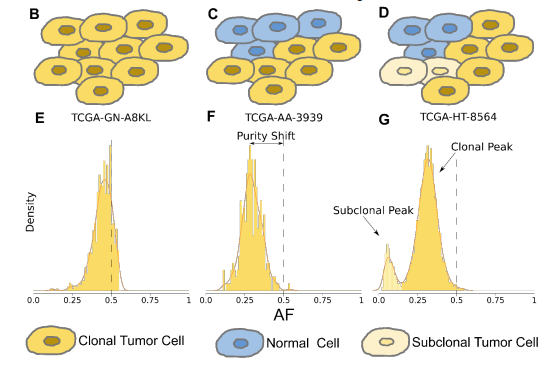
\includegraphics[width=0.5\linewidth]{peaks.png}
    \caption{\label{fig:peaks}Peaks shift for a clonal tumor cell population and some mixed populations. Considering two genomic locations, healthy cells have genotype AA-AA, clonal tumor cells AB-AA and subclonal tumor cells AB-AB, where B is the alternative allele associated with a somatic point mutation}
\end{figure}

The distribution of allelic fractions of the clonal population only is symmetric, with the main peak around 0.5. A mixed population of clonal tumor and normal healthy cells shows a shifted peak. The distance from 0.5 to the peak is proportional to the fraction of normal cells, because normal cells contribution moves the peak towards the side from the center (purity shift displayed in \ref{fig:peaks}. A subclonal point mutation is identified with a second peak towards 0, because its allelic fraction is probably far distant from 0.5.

\section{TPES (Tumor Purity Estimation)}
\textit{Alessio Locallo (Demichelis' student, 2019)}\\

\begin{figure}[!ht]
\centering
    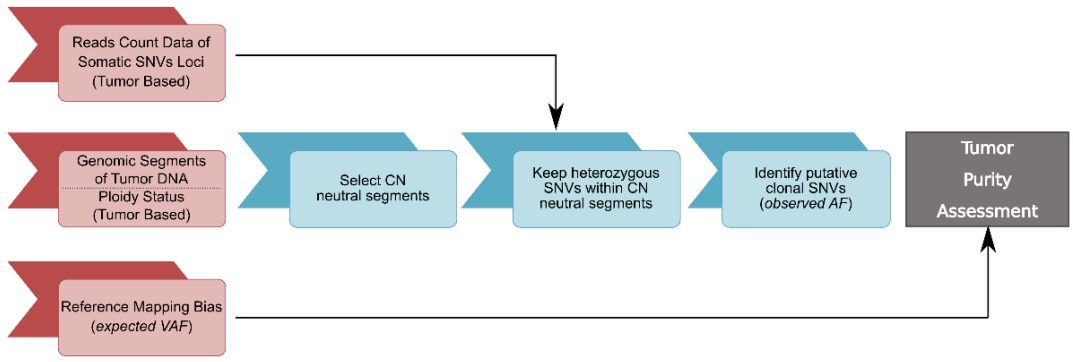
\includegraphics[width=0.7\linewidth]{tpes.png}
    \caption{\label{fig:tpes}Workflow of the TPES algorithm}
\end{figure}

It is important to consider the \textbf{Reference Mapping Bias}: a polymorphic locus carrying a non-reference base is less likely to be mapped during the alignment process. With a perfect SNV (clonal, monoallelic, in highly pure tumor), allelic fraction will not be 0.5 because the aligner considers the variation as an error and sometimes discards the read containing it: some signal is lost.\\

TPES steps:
\begin{itemize}
    \item \textbf{Selection of CN-neutral segments}: point mutations that are flat in terms of copy-number are perfect for flat genomes and easier to deal with. This is the first filter implemented by this tool: a threshold is set on the log2 of the tumor over the normal.
    \item When considering the \textbf{allelic fractions} of all the somatic mutations of whole genome, a major peak is expected around 0.5 (expected VAF). Other peaks can be originated from things that escaped the previous filter or from monoallelic mutations with copy-neutral LOH (loss of heterozygosity): in this case the allelic fraction results doubled. So another threshold on allelic fraction is needed (maxAF=0.55)
    \item Identification of \textbf{putative clonal SNVs}: the peak closer to 0.5 is the most useful to determine tumor purity. The others are related to subclonal events.
\end{itemize}

With enough point mutations and after peaks identification, purity is assessed with the following equation:
\[ 1-purity = admixture = 1-\frac{observedVAF}{expectedVAF} \]

\section{How many SNVs are needed to assess tumor purity?}

The number of SNVs changes for each tumor type, so not all tumor types guarantee enough SNVs. The minimum number of SNVs needed to obtain reliable results can be assessed with a \textbf{comparative analysis}. The Spearman's correlations between the results of two different purity calling algorithms uding decreasing number of SNVs are computed. The subsampling approach (which SNVs to consider?) is to subsample the SNVs as many time as possible to have higher confidence on the results. At each iteration, as many samples as possible are used, but the number decreases when the number of SNVs increases.

The computations determined 10 as the minimum number of SNVs needed to infer tumor purity. With this number, tumor was detected in 80\% of samples by combining TPES and CLONET (CN-based). The 20\% could be tumor-free or not detected samples. Since both SNVs and CN based methods failed, this 20\% could be possibly detected with methylation.

\begin{figure}[!ht]
\centering
    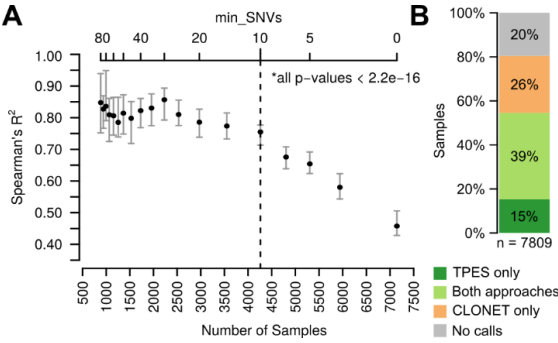
\includegraphics[width=0.7\linewidth]{comparative.png}
    \caption{\label{fig:comp}\textbf{A}) Correlation between two purity estimating algorithms (TPES and CLONET) with decreasing number of SNVs considered. \textbf{B}) Percentages of samples where tumor purity was assessed by the two tools (TPES considering with 10 SNVs)}
\end{figure}


\section{Comparison between purity callers}

TPES was compared to other tools that do the same thing but with a range of different methodologies: good correlation between the results was found, in particular with the CN-based algorithms. This shows that genomics is more reproducible in general to assess purity, while methods relying for example on image analysis give different results.

The best solution to assess tumor purity is to couple and CN-based and a SNV-based approach: some samples are only detected by one of the two so a combination gives the best results globally.

\section{Pros and Cons of SNVs-based tumor purity assessment}
Pros:
\begin{itemize}
    \item Best-suited for CN neutral tumor genomes
    \item Applicable to a range of NGS techniques
    \item Fast and low demanding in terms of computational resources
    \item TPES is available as R package on CRAN
\end{itemize}
Limitations:
\begin{itemize}
    \item Needs a reasonable number of putative clonal somatic heterozygous SNVs per sample
    \item  Sensible to subclonal cell populations which could influence clonal peak detection
\end{itemize}
